\documentclass[11pt,a4paper,twoside,openright]{report}                          % openright:  Makes chapters begin only on right side. twoside:    print on both sides.

\usepackage[a4paper,left=3.5cm, right=2.5cm, top=3.5cm, bottom=3.5cm]{geometry}
\usepackage[english]{babel}                                                     % Sets language, used for smart cap.
\usepackage{graphicx}                                                           % Makes it possible to import external graphics.
\usepackage[utf8x]{inputenc}                                                    % sets encoding to UTF8.
\usepackage[square, numbers]{natbib}                                            % Author-year & numbered references + other bibliography styles.
\usepackage{listings}	                                                        % Typeset programming code
\usepackage{verbatim}					                                        % show code, commands, ...
\usepackage[hyphens]{url}
\usepackage[breaklinks]{hyperref}
\usepackage{url}						                                        % Package that adds 'real' urls. with \url. 
\usepackage[small,bf,hang]{caption}                                             % Improves styling captions.
\usepackage[final]{pdfpages}                                                    % import PDFs
\usepackage{pslatex}					                                        % Other fonts than default
\usepackage{lipsum}                                                             % Load lorem ipsum texts with \ipsum, see docs.
\usepackage{sectsty}					                                        % Better styling control of section headers & chapters.
\usepackage{csquotes}                                                           % Support for quoting.
\usepackage{float}                                                              % Required to position figures
\usepackage{style-template}                                                     % Import style template.
\usepackage{wrapfig}                                                            % Package that helps positioning figures.
\usepackage{appendix}                                                           % Provide more commands to control the appendices
\usepackage{glossaries}                                                         % Package used to create glossary
\usepackage{minted}                                                             % Code highlighting
\usepackage{booktabs}                                                           % Package that helps to create beautiful tables
\usepackage{fontawesome5}                                                       % Font awesome icons.
\usepackage{adjustbox}                                                          % Scale tables to page width.

\makeglossaries                                                                 % Required before the first glossary entry.

\graphicspath{{figures/}}                                                       % Set default search path for figures (./figures).
\nocite{*}                                                                      % Show references that are not cited specifically.

\addto\captionsenglish{\renewcommand{\contentsname}{Table of Content}}          % Change title above ToC to Table of Content (default: Contents).

% Settings for appendices
\renewcommand{\appendixtocname}{List of appendices}                             % Change title for in ToC from 'appendix' to 'List of appendices'.

% Preface arguments
\acknowledgementspagetrue                                                       % Enable acknowledgment page.
\acknowledgements{acknowledgments}	                                            % preface.tex containing the preface content.
\abstractpagetrue                                                               % Enable abstract page.
\abstracts{abstract}		                                                    % abstract.tex containing abstract's content
\listoffigurespagetrue                                                          % Enable list of figures
\listoftablespagetrue                                                           % Enable list of tables
\listofglossariespagetrue                                                       % Enable glossaries
\listofglossaries{glossary}			                                            % glossary.tex containing list of abbreviations

% Variables Used in title page
\title{the recommended software to prototype large tabular data}                 
\subtitle{Comparative  Research}  
\institution{University College Howest}                                                 
\fieldOfStudy{Computer and Cybercrime Professional}                 
\releaseDate{June 2020}                                                                 
\author{Van Severen Emiel}                                                      % Author (can also be used throughout the document. If required.
\promoterAtype{Internal supervisor}                                             % Internal supervisor
\promoterAname{Mr. K. SYS}                                                      % Name internal supervisor
\promoterBtype{External promoter}                                               % Name External promoter
\promoterBname{Mr. P. VANCOMPERNOLLE}


\newglossaryentry{dma}
{
    name=DMA,
    description={DataMiner Agent is a single server in a DataMiner System, which has the ability to manage a certain number of devices and systems}
}

\newglossaryentry{dms}
{
    name=DMS,
    description={DataMiner System represents all the connected devices and systems within DataMiner}
}

\newglossaryentry{oss}
{
    name=OSS,
    description={Operations Support System is a computer system used in telecommunications service providers to manage their networks. It enables the service providers to monitor, control, analyse
    and manage the services on their network}
}

\newglossaryentry{kpi}
{
    name=KPI,
    description={Key Performance Indicator is a way of measuring a company's progress towards the goal it is trying to achieve}
}

\newglossaryentry{nms}
{
    name        = NMS,
    description = {Network Management System is a computer system designed for monitoring, maintaining and optimizing a network}
}
\newglossaryentry{hfc}{
    name        = HFC,
    description = {Hybrid Fibre-Coaxial is a term used by the telecommunications industry. A broadband network that combines optical fiber and coaxial cable to create broadband connections}
}

\newglossaryentry{wmi}{
    name        = WMI,
    description = {Windows Management Instrumentation is a set of specifications from Microsoft consolidating the management of devices and applications in a network of Windows computing systems. Meanwhile a new version has arisen called Windows Management Infrastructure (MI)}
}

\newglossaryentry{xml}{
    name        = XML,
    description = {e{X}tensible Markup Language is a markup language that defines a set of rules for encoding documents in a format that is both human-readable and machine-readable}
}

\newglossaryentry{bis}{
    name        = BIS,
    description = {Business Intelligence Software is a type of software created to retrieve, analyse, visualize and report data. The BIS is often used as support in making a wide range of business decisions},
}
\newglossaryentry{ui}{
    name        = UI,
    description = {User Interface is the point of human-computer interaction and communication in a device. This can include display screens, keyboards, a mouse and the appearance of a desktop. It is also the way through which a user interacts with an application or a website \cite{m-rouse}}
}
\newglossaryentry{viewport}{
    name        = viewport,
    description = {The viewport is the user's visible area of a web page. Depending on the device, this will vary. A mobile phone's viewport will be smaller than a computer screen's viewport}
}

\newglossaryentry{sql}{
    name        = SQL,
    description = Structured Query Language is a standardized programming language to manage and manipulate relational databases. 
}
%%%%%%%%%%%%%%%%%%%%%%%%%%%%%%%%%%%%%%%%%%%%%%%%%%%%%%%%%%%%%%%%%%%%%%%%%%%%%%%%%%%%%%%%%%%%%%%%%%%%%%%%%%%%%%%%%%%%%%%%%%%%%%%%%%%%%%%%%%%%%%%%%%%%%
%                                                           BEGIN DOCUMENT
%%%%%%%%%%%%%%%%%%%%%%%%%%%%%%%%%%%%%%%%%%%%%%%%%%%%%%%%%%%%%%%%%%%%%%%%%%%%%%%%%%%%%%%%%%%%%%%%%%%%%%%%%%%%%%%%%%%%%%%%%%%%%%%%%%%%%%%%%%%%%%%%%%%%%
\begin{document}
\selectlanguage{english}

\preface                            % contains everything until the chapters start

\chapter{Skyline Communications}
\section{Brief history}

Skyline Communications was founded in 1985 by Mr. Leo. Vandenberghe. The company started off as a local distributor of telecom infrastructure. In the mid 90's, Skyline Communications also emerged as a supplier of network management solutions. After the turn of the century, Skyline Communications has repositioned itself and became a software vendor. Over the years it became clear that the complexity of the broadcast and telecom systems was only increasing. They introduced their revolutionary \dm network management solutions.

Shortly thereafter Mr. Leo. Vandenberghe passed the company on to his progeny. In the following years Ben Vandenberghe took on the role of CEO, Bert Vandenberghe became CTO and Frederik Vandenberghe became CFO. 

\section{Current position}

Currently Skyline Communications has over 300 employees with new employees joining almost every day. 
The company has branches in Singapore, Lisbon, Miami, with its HQ located in Izegem. 
The HQ is a brand new building called the Skyline Park. (\url{https://skylinepark.be/})

Among the customers we find almost all the major media groups worldwide (e.g. BBC, SKY), a number of telecom giants (e.g. Verizon) but also the European Space Agency, the European Parliament, to name but a few. 

We can say with full conviction that Skyline Communications has taken a leading position in the market of vendor-independent network management solutions in the \gls{hfc} broadband, broadcast, satellite and telecom industry. 

\section{\dm platform}

The \dm platform has been an ongoing work in progress for over \underline{20 years}. It is therefore very extensive. Below are a few of the core components:


\subsection{DataMiner Driver}
A Driver, often referred to as a \textit{protocol}, is an XML file that allows the DMA to communicate with a device in the system. The file describes which information is retrieved and how it is processed, how to actively sampling its status, display real-time data, alarm thresholds, parameter labels..

Since the drivers are designed in an XML markup format, \underline{any} third-party is able to develop these drivers. Skyline even provides training sessions for companies to create their own protocols. This is called the  

An example of a protocol is called Microsoft Platform. The protocol makes use of \gls{wmi} to communicate and remotely manage Windows devices. For reference, this XML file is approximately 12000 lines of code. To this day Skyline supports 5500+ drivers. 


\subsection{DataMiner Agent}

A DataMiner Agent or \textit{\gls{dma}} is a piece of hardware running the DataMiner software. It makes use of DataMiner Drivers to aggregate data from various devices and systems that are part of the network. In practice you won't have one DMA, but a cluster of DMA's automatically acting as one big \textit{\gls{dms}}.  

\subsection{DataMiner Cube}
The DataMiner Cube is the main user interface to connect to a DMA. The broad range of functionalities allow you to manage very complex telecom environments. It offers alarm thresholds, performance management tools, user collaboration capabilities, correlation strategies,  automation scripts, redundancy groups and many other features. 

\subsection{DataMiner Dashboards}
 DataMiner Dashboards is one of the many standalone web applications. It can be used to visually track, analyse all kinds of data on a dashboard. The dashboards can be completely user-defined. Operators can create custom dashboards to their own needs. Since the information is a web application it is accessible on every device, even on mobile. A screen capture of a dashboard can be found in \autoref{dataminer_dashboards}.
 
 
\subsection{Other Applications}
For those who are interested, here is a list of other applications. DataMiner Monitoring, DataMiner Ticketing, DataMiner Jobs, DataMiner Collaboration, DataMiner Catalog. 

You can find a more detailed explanation on: \url{https://skyline.be}


\chapter{Research topic}

\section{Origin}
As stated in \autoref{dataminer-dashboards-information}, my internship revolves around the development within the DataMiner Dashboards application, more specifically, the usage of the generic interface. Although the generic interface provides little to no contribution to the outcome of the paper, it is the origin of the research and it provides a very interesting insight on how a large company solves certain problems. You can find a detailed explanation in \autoref{app:generic-interface}.

Currently the Dashboards application has no data analytics layer. Data can be visualized but can not be filtered or aggregated. There are utilities that provide filtering or aggregations in the front end but this is not a solution for large data sets as it is extremely slow and insufficient.
  
\section{Main research question}
The generic interface returns data in a flat table. It would be nice if this could be immediately visualized. A table is a rather simple but yet very powerful way to visualize information. But due to the large amount of data that Skyline's customers have to deal with, these tables often exist out of thousands of rows and dozens of columns, even after they are filtered. A table with these amounts of data quickly becomes inconvenient, obscure and generally not worth using. 

But how can we visualize large tabular data without sacrificing usability? This requires extensive user testing! A common technique is called prototyping. See \autoref{sec:prototyping}. We can create prototypes using prototyping software. 

After testing some of these prototyping software, I couldn't find the appropriate software for this use case. So what is the best tool to create and test large tables and the functionalities that go with it? Is there a tool that supports all the features? Where do the current tools lack?

\textbf{Note:} Although the focus is on Skyline Communications' customers, the results will be applicable to other use cases.

\chapter{Theoretical explanation}

\section{User experience (design)}
The official definition of user experience is: 
\begin{displayquote}
    A person's perception and responses resulting from the use and/or anticipated use of a product, system or service. (ISO 9241-11:2018, subsection 3.15).
\end{displayquote}

User experience \underline{design} is about making the user's experience with the product the best it can be. People who are interested should be attracted, once they are using the product, their journey should be as easy and pleasant as possible. To expose the needs of the user we should discover the behaviours, motivations and needs of the customer through observation, task analysis and other types of user feedback.

\subsection{UX Process}
    \subsubsection{User Personas}
    User personas are fictional characters, which are created based upon research in order to represent the different user types that might use your service, product, site or brand. As of today four different perspectives regarding personas exist. Only \underline{three} are related to this research.
    
    \paragraph{The goal-directed perspective}
        This perspective focuses on what the typical user wants to do with the product. As a \autoref{ux} researcher you want to examine the process a user would prefer to utilise in order to achieve their objectives. The goal-directed perspective is beautifully displayed in \autoref{fig:goal-directed-persona-perspective}. Author/Copyright holder: Smashing Magazine.
        \begin{figure}
            \centering
            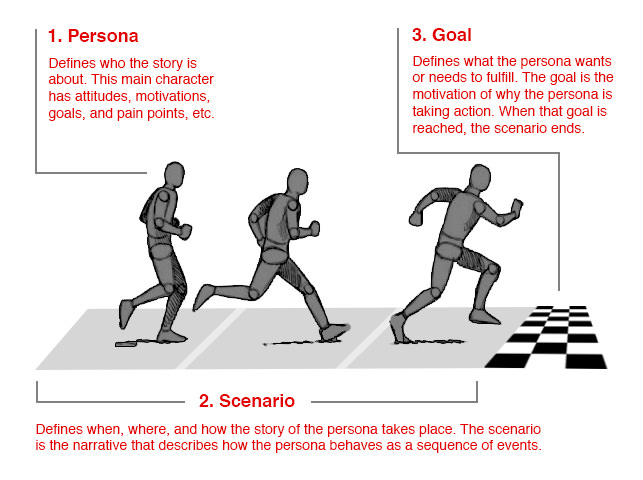
\includegraphics[scale=0.5]{goal-directed-perspective.jpg}
            \caption{Goal-directed persona perspective}
            \label{fig:goal-directed-persona-perspective}
        \end{figure}
    \paragraph{The role-based perspective}
    The role-based perspective is also a goal-directed perspective, but mainly focused on behavior. They are mainly focused on the role of the user inside the organization. A role-based persona should give an answer to the questions below.
    \begin{itemize}
        \item{Where will users use our product?}
        \item{What is the purpose of the product?}
        \item{What business objectives are required and what can be achieved with them?}
        \item{Which people will be impacted by its role?}
        \item{What kind of functions are being served..?}
    \end{itemize}
    
    \paragraph{The engaging perspective}
    Through an understanding of characters and stories, it is possible to create a realistic description of fictitious people. The engaging personas are designed so that the designers who use them can become more engaged with them. The more people engage with the persona and see them as 'real', the more likely they will be to consider them during the process design.
    
    \subsubsection{User Stories}
    Stories capture the characteristics of the design space and audience that designers and engineers need to understand to build a complete and useful software experience. A story is a design communication tool that transcends the cultural divides of multidisciplinary teams and intertwines a technology with its user's goals. This article describes how stories are powerful tools in software design, defines the elements that make a compelling story, and presents the use of stories at IBM from the authors' experience. It also explores the benefits at each phase of the design process and how stories evolve throughout the design process.
    \paragraph{User Flows}
    explanation about what user flows are
    
    \subsubsection{Research}
    \paragraph{mockups / wireframes}
    
    \subsubsection{Design}
    just some basic information about design
    
    \subsubsection{Implementation}
    information about the implementation
    
    \subsubsection{Evaluation}
    \paragraph{User feedback}
    \paragraph{UI audit reports}
    
\section{Data Analysis}
    \subsection{What is data analysis?}
    \subsection{What types of data analysis exists?}

\section{Generic interface}
    A major part of software engineering is building components that not only have a well-defined and consistent APIs, but are also very  \underline{reusable}. 
    \subsection{What is a generic interface}
    
\chapter{Comparing prototyping software}

\section{Introduction}
Before you create prototypes it is important to understand who your users are and what issues they have. I have worked out user personas, use cases and more for Skyline Communications' customers..You can find these in \autoref{app:skyline-communication}.

\section{Prototyping software}
The prototyping software business has become a very competitive market, particularly in the last 5 to 10 years. Every company needs/wants a website. Chances are that your local bakery and butchery have one. Although these software tools are rapidly improving and adding new features persistently, until now they are still mostly limited to the visual design.

What is the best tool for creating large tables and the functionalities that go with that? Do the current software tools support these features or where are they lacking? Below you can find the tools that are being compared:
\begin{itemize}
    \setlength\itemsep{-0.5em}                                    
    \item {Adobe XD}
    \item {Figma}
    \item {Invision Studio}
    \item {Framer}
    \item {Axure RP}
    \item {Sketch}
\end{itemize}

Mind you, Sketch had been adopted as the industry standard for years. But excellent competitions changed this. Currently Its market position is being jeopardized. Although Sketch has been immensely popular, it forces you to use macOS. Since I do not own a device with macOS, it can not be tested properly. Sketch is too big of a player to leave out. The results of Sketch are discussed less extensively, without hands on testing. 

\section{Properties and features}
To compare the tools, I have carefully selected criteria. this includes both general criteria and criteria specifically required to visualize large tabular data. Below are the criteria that will be discussed in \autoref{chap:research-criteria}:  

    \begin{itemize}
    \setlength\itemsep{-0.5em}    
        \item{Popularity}
        \item{Price}
        \item{Platform}
        \item{Collaboration}
        \item{Sharing}
        \item{Community}
        \item{Handoffs}
        \item{Horizontal scroll bar}
        \item{Click events}
        \item{View lock}
        \item{Context menu}
    \end{itemize}
\chapter{Practical: UX Design}

\section{Understand the user}
    \subsection{User personas}
        user persona here
    \subsection{User stories}
        user stories here
    \subsection{Use cases}
        use cases here

\section{Research}
    \subsection{Competitors}
        \subsubsection{Tableau}
        tableau information here
        \subsubsection{other?}
        other competitors here
    \subsection{Analyse latest ux trends}
    analysis here
    \subsection{Fit in current design}
    fit to current design here
    
\section{Sketch}
    \subsection{wireframes/mockups}
    wireframes here
    \subsection{user flows}
    userflows here
    
\section{Design}
    \subsection{evolution of design}
    evoluation of design

\section{Implementation}
    eventueel hier zeggen dat dit een groot onderdeel is en wordt behandeld in het volgende hoofdstuk

\section{Evaluation}
    \subsection{User Feedback}
    user feedback here
    \subsection{UI Audit reports}
    ui audit reports here
    

\chapter{backup}
\chapter{Conclusion}
\chapter{Critical reflection}

\nocite{*}                          % Prints all references even if they are not cited.
\raggedright                        % Solves an issue with the spacing in the bibliography.
\bibliographystyle{apalike} 
\bibliography{bibliography}         % Handles references.bib

\noappendicestocpagenum             % Remove pagenumber of ToC entry.
\addappheadtotoc                    % Add Entry to ToC. 
\appendix                           % Files imported after this tag will be seen as appendixes
\chapter{DataMiner Dashboards}
\label{dataminer_dashboards}

For your information, Last year Skyline Communications organized an event called DataMiner Inspire. Customers from all over the world descend to Izegem to catch a glimpse of what Skyline has to offer in the (nearby) future. Among the guests, all the major players in the media industry. Including representatives of Al Jazeera, Discovery Channel, Sky and OneWeb. The latter company is currently launching more than a \underline{1000 satellites} for the construction of a global internet system.

The screen capture was taken from a demo dashboard used throughout the event to show the capabilities of dashboards application. Mind you, these dashboard components were not ready for production and were build specifically for the event. 
\begin{center}
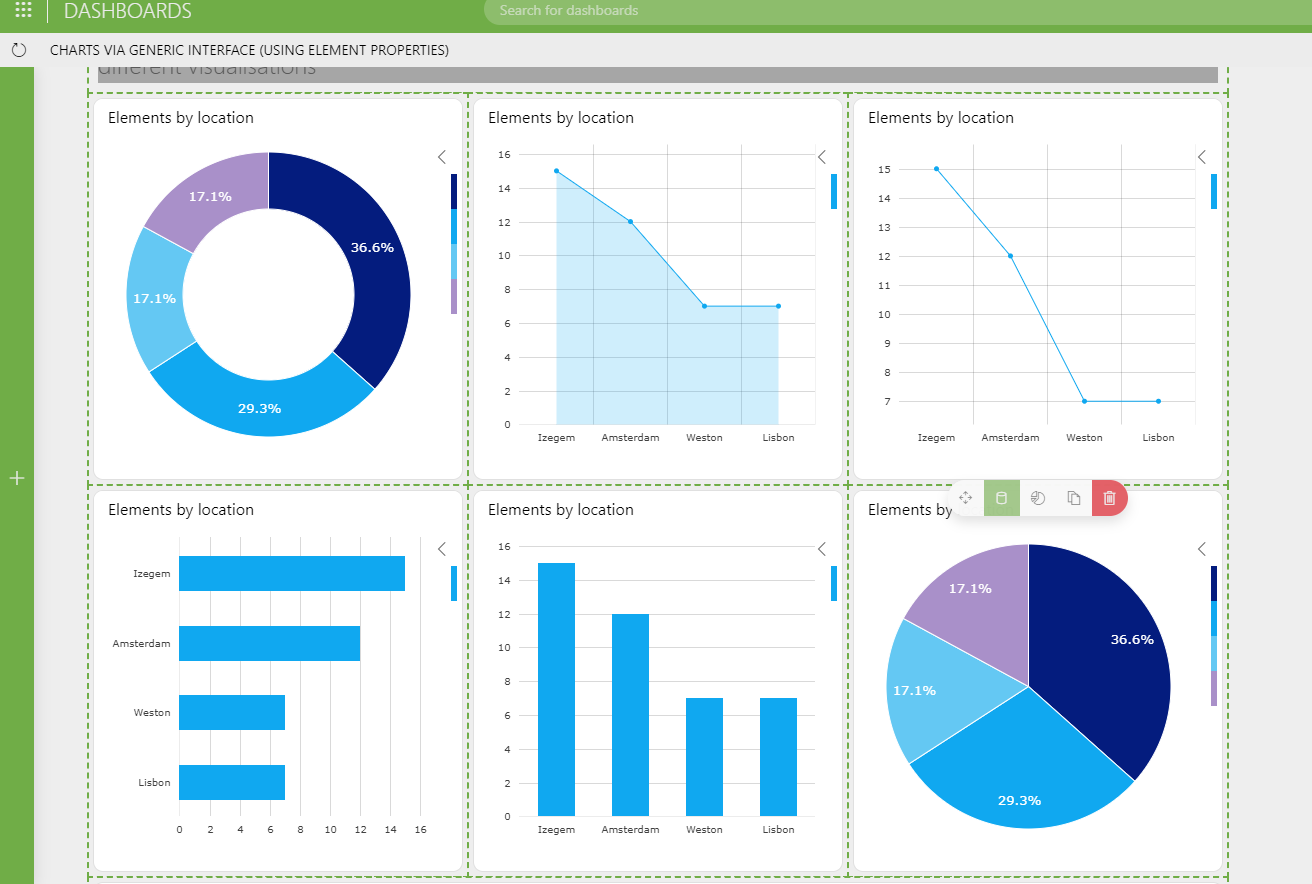
\includegraphics[scale=0.5]{dashboards}
\end{center}

\chapter{User personas}\label{user_personas}

\begin{center}
\includegraphics[scale=0.5]{figures/user-persona-1.png}
\end{center}

\begin{center}
\includegraphics[scale=0.5]{figures/user-persona-2.png}
\end{center}

\begin{center}
\includegraphics[scale=0.5]{figures/user-persona-3.png}
\end{center}
\chapter{Research Skyline Communication}\label{app:skyline-communication}


\section{User Personas}
Below in \autoref{fig:user-persona-1}, \autoref{fig:user-persona-2}, \autoref{fig:user-persona-3}, you can see the user personas that represent Skyline communications' customers. More specifically those who use the DataMiner Dashboards application.

\subsection{Gitlab}
A company that uses user personas magnificently is Gitlab. Gitlab has created an entire, fictional company where the employees represent its customers. To give you an idea, Gitlab has created user personas for a compliance manager, product manager, development team lead, product designer, software developer, devOps Engineer, systems administrator, security analyst and many more. Each persona has its own job summary, motivations, frustrations, challenges...

Here's a link to Gitlab's user personas: \url{https://about.gitlab.com/handbook/marketing/product-marketing/roles-personas/#personas}


\begin{figure}[H]
        \centering
        \includegraphics[scale=0.5]{figures/user-persona-1.png}
        \caption{User persona 1}
        \label{fig:user-persona-1}
    \end{figure}
    
\begin{figure}[H]
    \centering
    \includegraphics[scale=0.5]{figures/user-persona-2.png}
    \caption{User persona 2}
    \label{fig:user-persona-2}
\end{figure}

\begin{figure}[H]
    \centering
    \includegraphics[scale=0.5]{figures/user-persona-3.png}
    \caption{User persona 3}
    \label{fig:user-persona-3}
\end{figure}

\section{Use cases}
        \begin{itemize}
            \setlength\itemsep{-0.5em}                                    
            \item {As a user I can position my data, so that the most relevant data is immediately visible.}
            \item {As a user I can control the width of a column, so that they take up less space.}
            \item {As a user I can }
        \end{itemize}
    
    \section{DataMiner Dashboards competitors}
        As a company you don't always have to reinvent the wheel. It can be very useful to see how competitors solve certain problems. But who are Skyline DataMiner Dashboards' biggest competitors? How do they visualize large tabular data?
        
        \subsection{Tableau}
        \subsubsection{What is Tableau?}
        Tableau is the leading Business Intelligence software (\gls{bis}). With Tableau users can easily retrieve, analyse, transform and report data. It enables users to effortlessly visualize data regardless of its format. The software is very easy to use and does not require any knowledge of coding. What makes Tableau so unique compared to others is their quality of data visualizations and self-service analytics. It was found in 2003 by Christian Chabot, Pat Hanrahan and Chris Stolte. In August 2019, Tableau was acquired by \href{https://www.salesforce.com/}{Salesforce} for a stunning 15 Billion dollars.
        
       \subsubsection{Table} 
        \subsection{Power BI}
        \subsubsection{What is Power BI?}
        Power BI is a business intelligence software developed by Microsoft. It is completely integrated with Office 365, which makes it very easy to import data from applications like Excel. Power BI has only been released in 2014 but was immediately seen as a competitor for tableau. Compared to Tableau, power Bi has a free desktop applications for individuals.
        
        \subsubsection{Table}
        
        \subsection{Kibana}
        \subsubsection{What is Kibana?} 
        Elastic is a search company 
        Kibana is a browser-based analytics and search dashboard for Elasticsearch, a powerful, open source, search engine. Although it is classified as a Monitoring tool, while the other discussed software are business intelligence software, Kibana provides very appealing and thoughtful visualizations.
        \subsubsection{Table}
        
        \subsection{Other}
        \begin{itemize}
            \setlength\itemsep{-0.5em}                                    
            \item{Oracle BI}
            \item{Geckoboard}
            \item{Sisense}
            \item{Dundas Data Visualization}
            \item{SAP Business Objects}
            \item{Domo}
        \end{itemize}
   
\chapter{User experience example}\label{app:user_experience}
\section{Tomato ketchup bottle}
Around 1889 Heinz introduced its octagonal glass ketchup bottle. The iconic glass bottle was their staple for over a hundred years. But in the world of user experience research not the glass bottle, but the current plastic bottle is known as one of the greatest innovations since the invention of semiconductors. (\textit{slightly exaggerated})

\subsection{Innovations}
Although Heinz had no intention to reinvent their ketchup bottle, it was determined to better understand how people were consuming its ketchup at home. 
The company did an extensive market-research in which researchers visited ordinary families and watched the way they used their ketchup. Something remarkable happened. Something that probably exceeded their greatest expectations.

Casey Keller, who was the chief growth offer for Heinz at the time, said: 

\begin{displayquote}
    \textit{
    "I remember sitting in one of those households, There was a three-year-old and a six-year-old, and what happened was that the kids asked for ketchup and Mom brought it out. It was a forty-ounce bottle. And the three-year-old went to grab it himself, and Mom intercepted the bottle and said, 'No you are not going to do that.' She physically took the bottle away and doled out a little dollop. You could see that the whole thing was a bummer."}
    \cite{Gladwell2009}
\end{displayquote}

Researchers had already discovered that children consume approximately 60\% more ketchup than an adult. But now, they found out that their biggest consumers, children, did not have direct access to the bottle. For as long as the parents are in control they would always restrain the consumption levels. 

The result was a so called 'EZ Squirt bottle'. This is a bottle completely made out of plastic with a cone-shaped tip. After thoroughly analysing the families that used this new bottle, it turned out to be a great success. The new ketchup bottle led to a consumption growth of 12\%!

Heinz did not stop there, they continued reinventing their bottle. In the beginning of the 21st century, after the sales were down, Heinz decided to conduct another user research. The researchers concluded that consumers struggled to get the leftovers out of the bottle. Instead of buying a new bottle, they kept using the leftover ketchup they tried to squeeze out, often this was less than they wanted. Getting the leftovers out was unpleasant and often a messy task. To fight this, people often stored their bottle upside down in the refrigerator. 

Again, Heinz came up with a great solution. They decided to turn the bottle over. And so, the current Heinz upside-down ketchup bottle was born.
You can see the result in \autoref{fig:heinz-ketchup-bottle}. The figure is downloaded from \url{https://www.ventera.com/sites/default/files/Heinz.png}

\begin{figure}[h!]
\centering
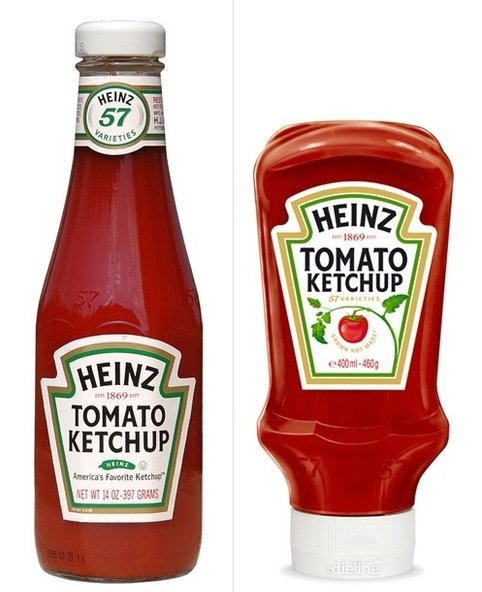
\includegraphics[scale=0.2]{figures/ketchup.png}
\caption{Heinz's tomato ketchup bottle before and after the innovation.}
\label{fig:heinz-ketchup-bottle}
\end{figure}

\chapter{Google Trends results}\label{app:google-trends}

\section{Interest by region and rising related queries }
    \begin{figure}[H]
        \centering
        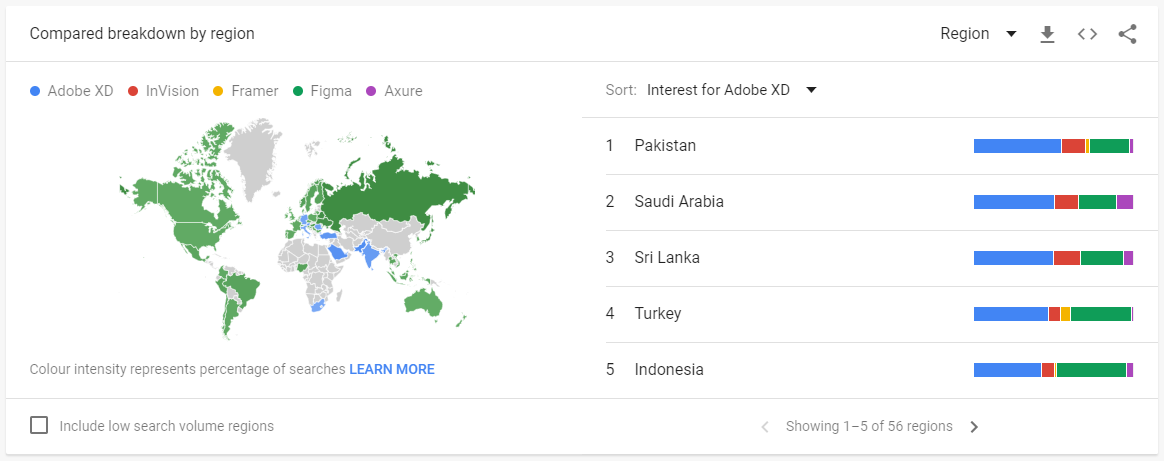
\includegraphics[scale=0.4]{figures/trends/adobe-xd-region.png}
        \caption{Adobe XD regional results}
        \label{app:google-trends-region-adobe-xd}
    \end{figure}
   
    \begin{figure}[H]
        \centering
        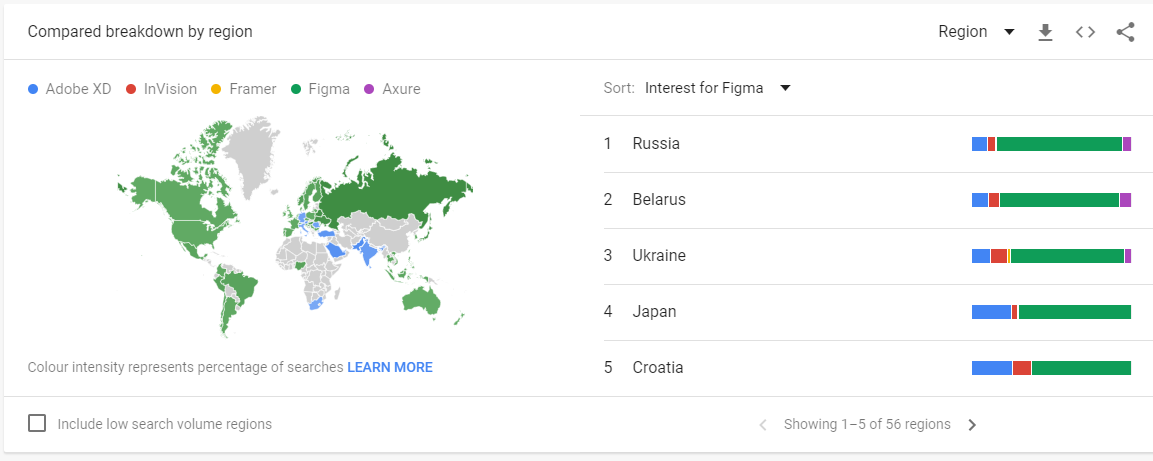
\includegraphics[scale=0.4]{figures/trends/figma-region.png}
        \caption{Figma regional results}
        \label{app:google-trends-region-figma}
    \end{figure}
   
    \begin{figure}[H]
            \centering
            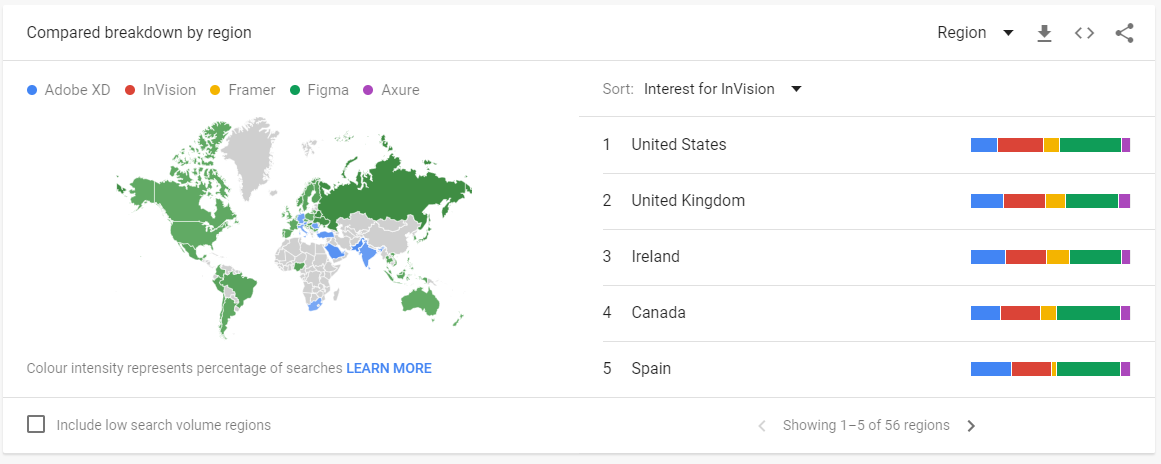
\includegraphics[scale=0.4]{figures/trends/invision-region.png}
            \caption{Invision regional results}
            \label{app:google-trends-region-invision}
    \end{figure}

    \begin{figure}[H]
        \centering
        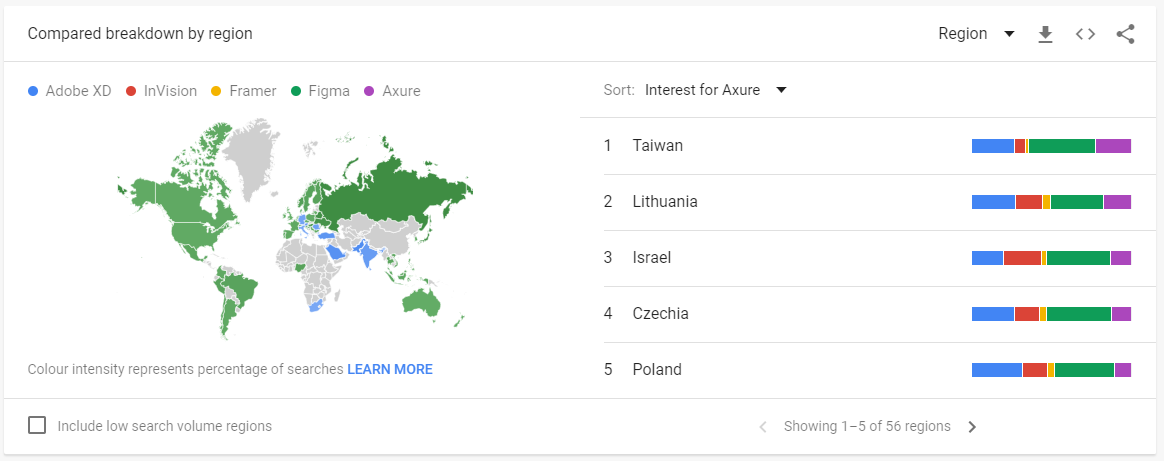
\includegraphics[scale=0.4]{figures/trends/axure-region.png}
        \caption{Axure regional results}
        \label{app:google-trends-region-axure}
    \end{figure}

    \begin{figure}[H]
        \centering
        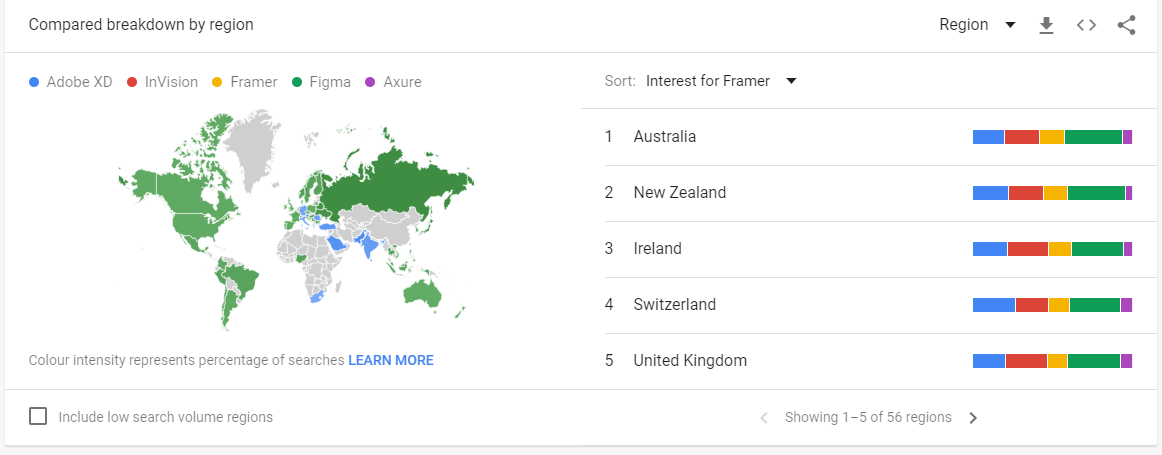
\includegraphics[scale=0.4]{figures/trends/framer-region.png}
        \caption{Framer regionional results}
        \label{app:google-trends-region-framer}
    \end{figure}
   
   \section{Related queries} 
    \begin{figure}[H]
        \centering
        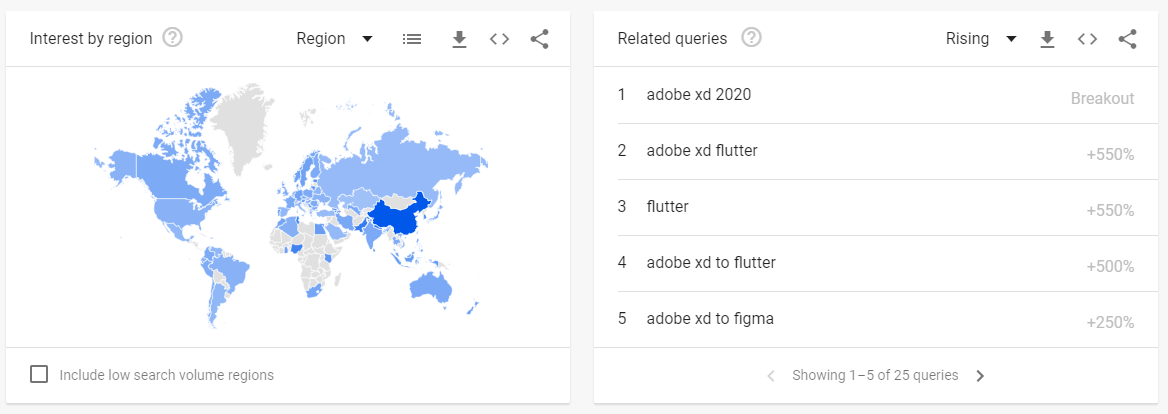
\includegraphics[scale=0.4]{figures/trends/adobe-xd-queries.png}
        \caption{Adobe XD related queries results}
        \label{app:google-trends-queries-adobe-xd}
    \end{figure}
    
    \begin{figure}[H]
        \centering
        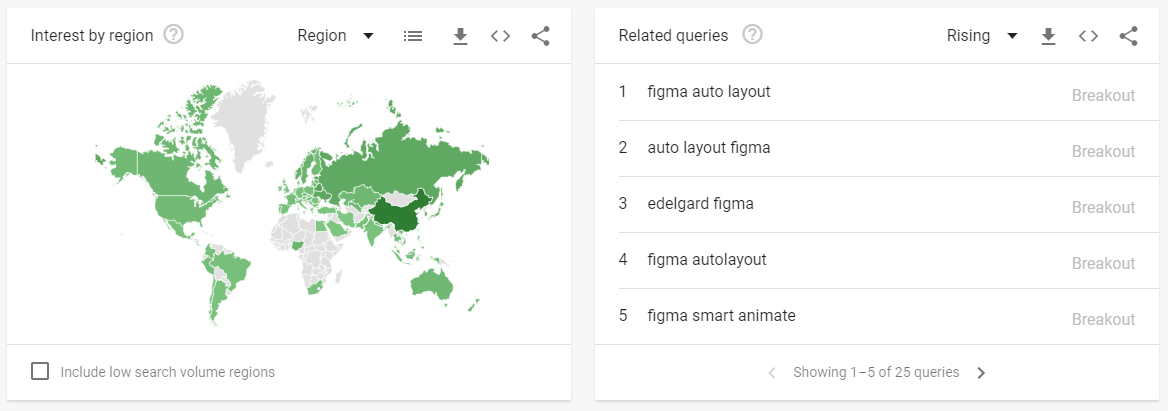
\includegraphics[scale=0.4]{figures/trends/figma-queries.png}
        \caption{Figma related queries results}
        \label{app:google-trends-queries-figma}
    \end{figure}
    
    \begin{figure}[H]
        \centering
        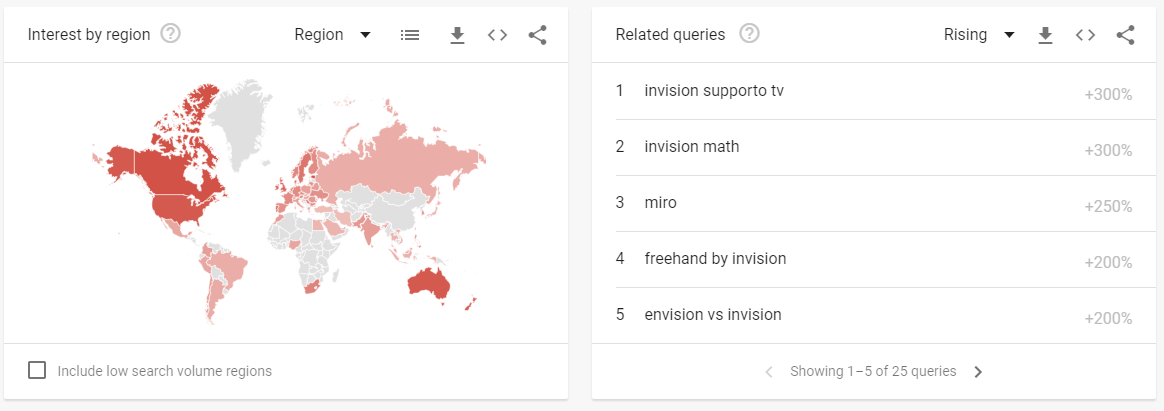
\includegraphics[scale=0.4]{figures/trends/invision-queries.png}
        \caption{Invision related queries results}
        \label{app:google-trends-queries-invision}
    \end{figure}
    
    \begin{figure}[H]
        \centering
        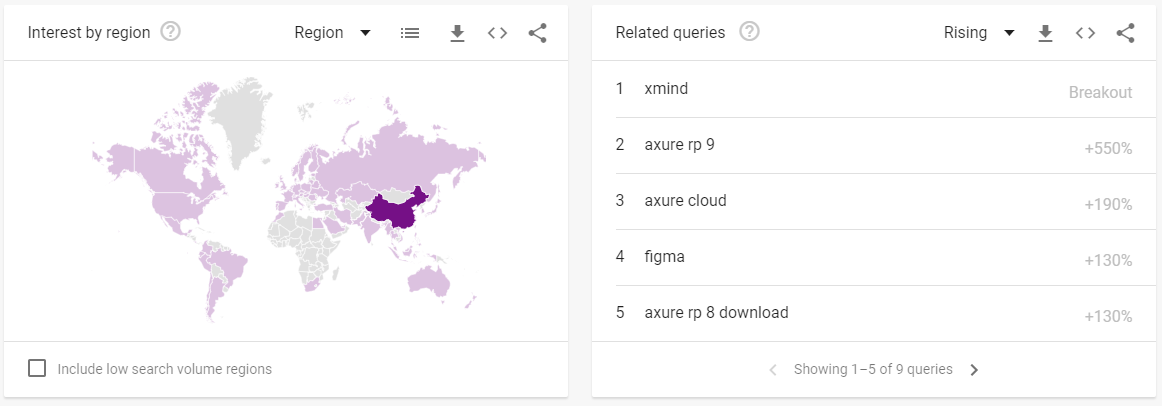
\includegraphics[scale=0.4]{figures/trends/axure-queries.png}
        \caption{Axure related queries results}
        \label{app:google-trends-queries-axure}
    \end{figure}
    
     \begin{figure}[H]
        \centering
        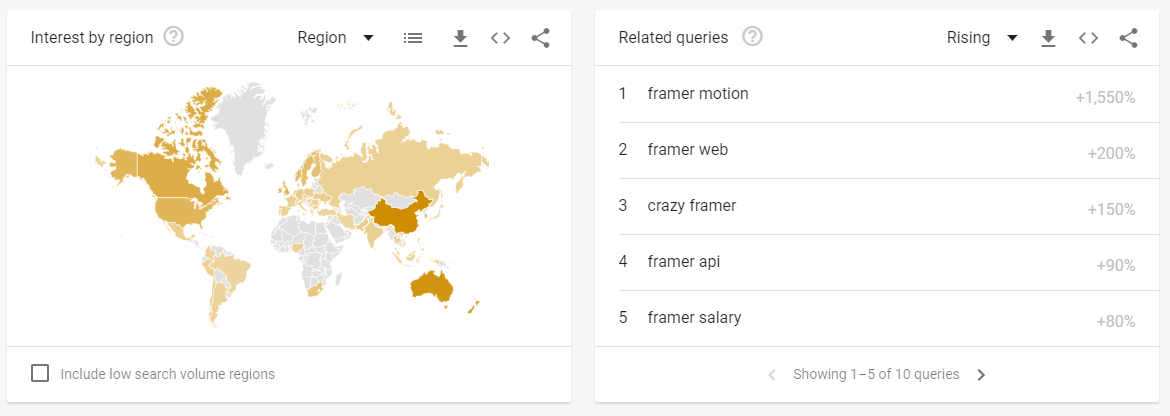
\includegraphics[scale=0.4]{figures/trends/framer-queries.png}
        \caption{Framer related queries results}
        \label{app:google-trends-queries-framer}
    \end{figure}
    

\end{document}
